% Options for packages loaded elsewhere
\PassOptionsToPackage{unicode}{hyperref}
\PassOptionsToPackage{hyphens}{url}
\PassOptionsToPackage{dvipsnames,svgnames,x11names}{xcolor}
%
\documentclass[
  letterpaper,
  DIV=11,
  numbers=noendperiod]{scrartcl}

\usepackage{amsmath,amssymb}
\usepackage{iftex}
\ifPDFTeX
  \usepackage[T1]{fontenc}
  \usepackage[utf8]{inputenc}
  \usepackage{textcomp} % provide euro and other symbols
\else % if luatex or xetex
  \usepackage{unicode-math}
  \defaultfontfeatures{Scale=MatchLowercase}
  \defaultfontfeatures[\rmfamily]{Ligatures=TeX,Scale=1}
\fi
\usepackage{lmodern}
\ifPDFTeX\else  
    % xetex/luatex font selection
\fi
% Use upquote if available, for straight quotes in verbatim environments
\IfFileExists{upquote.sty}{\usepackage{upquote}}{}
\IfFileExists{microtype.sty}{% use microtype if available
  \usepackage[]{microtype}
  \UseMicrotypeSet[protrusion]{basicmath} % disable protrusion for tt fonts
}{}
\makeatletter
\@ifundefined{KOMAClassName}{% if non-KOMA class
  \IfFileExists{parskip.sty}{%
    \usepackage{parskip}
  }{% else
    \setlength{\parindent}{0pt}
    \setlength{\parskip}{6pt plus 2pt minus 1pt}}
}{% if KOMA class
  \KOMAoptions{parskip=half}}
\makeatother
\usepackage{xcolor}
\setlength{\emergencystretch}{3em} % prevent overfull lines
\setcounter{secnumdepth}{4}
% Make \paragraph and \subparagraph free-standing
\ifx\paragraph\undefined\else
  \let\oldparagraph\paragraph
  \renewcommand{\paragraph}[1]{\oldparagraph{#1}\mbox{}}
\fi
\ifx\subparagraph\undefined\else
  \let\oldsubparagraph\subparagraph
  \renewcommand{\subparagraph}[1]{\oldsubparagraph{#1}\mbox{}}
\fi

\usepackage{color}
\usepackage{fancyvrb}
\newcommand{\VerbBar}{|}
\newcommand{\VERB}{\Verb[commandchars=\\\{\}]}
\DefineVerbatimEnvironment{Highlighting}{Verbatim}{commandchars=\\\{\}}
% Add ',fontsize=\small' for more characters per line
\usepackage{framed}
\definecolor{shadecolor}{RGB}{241,243,245}
\newenvironment{Shaded}{\begin{snugshade}}{\end{snugshade}}
\newcommand{\AlertTok}[1]{\textcolor[rgb]{0.68,0.00,0.00}{#1}}
\newcommand{\AnnotationTok}[1]{\textcolor[rgb]{0.37,0.37,0.37}{#1}}
\newcommand{\AttributeTok}[1]{\textcolor[rgb]{0.40,0.45,0.13}{#1}}
\newcommand{\BaseNTok}[1]{\textcolor[rgb]{0.68,0.00,0.00}{#1}}
\newcommand{\BuiltInTok}[1]{\textcolor[rgb]{0.00,0.23,0.31}{#1}}
\newcommand{\CharTok}[1]{\textcolor[rgb]{0.13,0.47,0.30}{#1}}
\newcommand{\CommentTok}[1]{\textcolor[rgb]{0.37,0.37,0.37}{#1}}
\newcommand{\CommentVarTok}[1]{\textcolor[rgb]{0.37,0.37,0.37}{\textit{#1}}}
\newcommand{\ConstantTok}[1]{\textcolor[rgb]{0.56,0.35,0.01}{#1}}
\newcommand{\ControlFlowTok}[1]{\textcolor[rgb]{0.00,0.23,0.31}{#1}}
\newcommand{\DataTypeTok}[1]{\textcolor[rgb]{0.68,0.00,0.00}{#1}}
\newcommand{\DecValTok}[1]{\textcolor[rgb]{0.68,0.00,0.00}{#1}}
\newcommand{\DocumentationTok}[1]{\textcolor[rgb]{0.37,0.37,0.37}{\textit{#1}}}
\newcommand{\ErrorTok}[1]{\textcolor[rgb]{0.68,0.00,0.00}{#1}}
\newcommand{\ExtensionTok}[1]{\textcolor[rgb]{0.00,0.23,0.31}{#1}}
\newcommand{\FloatTok}[1]{\textcolor[rgb]{0.68,0.00,0.00}{#1}}
\newcommand{\FunctionTok}[1]{\textcolor[rgb]{0.28,0.35,0.67}{#1}}
\newcommand{\ImportTok}[1]{\textcolor[rgb]{0.00,0.46,0.62}{#1}}
\newcommand{\InformationTok}[1]{\textcolor[rgb]{0.37,0.37,0.37}{#1}}
\newcommand{\KeywordTok}[1]{\textcolor[rgb]{0.00,0.23,0.31}{#1}}
\newcommand{\NormalTok}[1]{\textcolor[rgb]{0.00,0.23,0.31}{#1}}
\newcommand{\OperatorTok}[1]{\textcolor[rgb]{0.37,0.37,0.37}{#1}}
\newcommand{\OtherTok}[1]{\textcolor[rgb]{0.00,0.23,0.31}{#1}}
\newcommand{\PreprocessorTok}[1]{\textcolor[rgb]{0.68,0.00,0.00}{#1}}
\newcommand{\RegionMarkerTok}[1]{\textcolor[rgb]{0.00,0.23,0.31}{#1}}
\newcommand{\SpecialCharTok}[1]{\textcolor[rgb]{0.37,0.37,0.37}{#1}}
\newcommand{\SpecialStringTok}[1]{\textcolor[rgb]{0.13,0.47,0.30}{#1}}
\newcommand{\StringTok}[1]{\textcolor[rgb]{0.13,0.47,0.30}{#1}}
\newcommand{\VariableTok}[1]{\textcolor[rgb]{0.07,0.07,0.07}{#1}}
\newcommand{\VerbatimStringTok}[1]{\textcolor[rgb]{0.13,0.47,0.30}{#1}}
\newcommand{\WarningTok}[1]{\textcolor[rgb]{0.37,0.37,0.37}{\textit{#1}}}

\providecommand{\tightlist}{%
  \setlength{\itemsep}{0pt}\setlength{\parskip}{0pt}}\usepackage{longtable,booktabs,array}
\usepackage{calc} % for calculating minipage widths
% Correct order of tables after \paragraph or \subparagraph
\usepackage{etoolbox}
\makeatletter
\patchcmd\longtable{\par}{\if@noskipsec\mbox{}\fi\par}{}{}
\makeatother
% Allow footnotes in longtable head/foot
\IfFileExists{footnotehyper.sty}{\usepackage{footnotehyper}}{\usepackage{footnote}}
\makesavenoteenv{longtable}
\usepackage{graphicx}
\makeatletter
\def\maxwidth{\ifdim\Gin@nat@width>\linewidth\linewidth\else\Gin@nat@width\fi}
\def\maxheight{\ifdim\Gin@nat@height>\textheight\textheight\else\Gin@nat@height\fi}
\makeatother
% Scale images if necessary, so that they will not overflow the page
% margins by default, and it is still possible to overwrite the defaults
% using explicit options in \includegraphics[width, height, ...]{}
\setkeys{Gin}{width=\maxwidth,height=\maxheight,keepaspectratio}
% Set default figure placement to htbp
\makeatletter
\def\fps@figure{htbp}
\makeatother

\KOMAoption{captions}{tableheading}
\makeatletter
\makeatother
\makeatletter
\makeatother
\makeatletter
\@ifpackageloaded{caption}{}{\usepackage{caption}}
\AtBeginDocument{%
\ifdefined\contentsname
  \renewcommand*\contentsname{Table of contents}
\else
  \newcommand\contentsname{Table of contents}
\fi
\ifdefined\listfigurename
  \renewcommand*\listfigurename{List of Figures}
\else
  \newcommand\listfigurename{List of Figures}
\fi
\ifdefined\listtablename
  \renewcommand*\listtablename{List of Tables}
\else
  \newcommand\listtablename{List of Tables}
\fi
\ifdefined\figurename
  \renewcommand*\figurename{Figure}
\else
  \newcommand\figurename{Figure}
\fi
\ifdefined\tablename
  \renewcommand*\tablename{Table}
\else
  \newcommand\tablename{Table}
\fi
}
\@ifpackageloaded{float}{}{\usepackage{float}}
\floatstyle{ruled}
\@ifundefined{c@chapter}{\newfloat{codelisting}{h}{lop}}{\newfloat{codelisting}{h}{lop}[chapter]}
\floatname{codelisting}{Listing}
\newcommand*\listoflistings{\listof{codelisting}{List of Listings}}
\makeatother
\makeatletter
\@ifpackageloaded{caption}{}{\usepackage{caption}}
\@ifpackageloaded{subcaption}{}{\usepackage{subcaption}}
\makeatother
\makeatletter
\@ifpackageloaded{tcolorbox}{}{\usepackage[skins,breakable]{tcolorbox}}
\makeatother
\makeatletter
\@ifundefined{shadecolor}{\definecolor{shadecolor}{rgb}{.97, .97, .97}}
\makeatother
\makeatletter
\makeatother
\makeatletter
\makeatother
\ifLuaTeX
  \usepackage{selnolig}  % disable illegal ligatures
\fi
\IfFileExists{bookmark.sty}{\usepackage{bookmark}}{\usepackage{hyperref}}
\IfFileExists{xurl.sty}{\usepackage{xurl}}{} % add URL line breaks if available
\urlstyle{same} % disable monospaced font for URLs
\hypersetup{
  pdftitle={Cellular neighborhoods: a useful and straightforward analysis framework},
  pdfauthor={Patrick Danaher},
  colorlinks=true,
  linkcolor={blue},
  filecolor={Maroon},
  citecolor={Blue},
  urlcolor={Blue},
  pdfcreator={LaTeX via pandoc}}

\title{Cellular neighborhoods: a useful and straightforward analysis
framework}
\author{Patrick Danaher}
\date{2024-10-17}

\begin{document}
\maketitle
\ifdefined\Shaded\renewenvironment{Shaded}{\begin{tcolorbox}[enhanced, interior hidden, borderline west={3pt}{0pt}{shadecolor}, sharp corners, boxrule=0pt, frame hidden, breakable]}{\end{tcolorbox}}\fi

\renewcommand*\contentsname{Contents}
{
\hypersetup{linkcolor=}
\setcounter{tocdepth}{3}
\tableofcontents
}
\hypertarget{introduction}{%
\section{Introduction}\label{introduction}}

The literature is becoming crowded with analysis tools employing
elaborate techniques (graphical neural networks, Fourier transforms,
hidden Markov random fields) to solve straightforward problems
(e.g.~spatial clustering or seeking spatially auto-correlated genes).
While these methods promise more optimal performance, simpler techniques
have a different virtue: they make analyses easier to understand, both
for analysts and for their eventual audiences. In this spirit, we
recommend ``cellular neighborhoods'' as an framework for diverse
analyses. This approach is easy to implement, straightforward to riff
on, and computationally efficient

Cellular neighborhood analysis begins with two steps:

\begin{enumerate}
\def\labelenumi{\arabic{enumi}.}
\tightlist
\item
  Define each cell's neighboring cells.
\item
  Create a new matrix encoding cells' ``spatial contexts''. To do this,
  we compute summaries of each cell's neighbors, reporting for example
  their average expression profile or the abundance of different cell
  types within them.
\end{enumerate}

\begin{figure}

{\centering 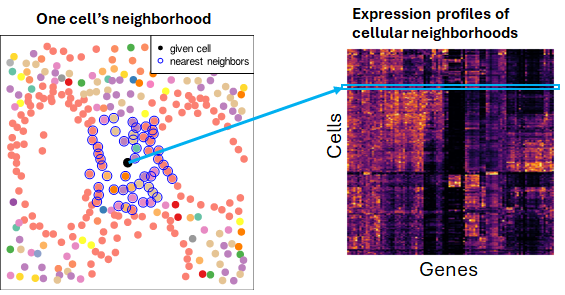
\includegraphics[width=1.2\textwidth,height=\textheight]{./figures/cartoon.png}

}

\caption{Left: example of a cellular neighborhood defined as a cell's 50
nearest neighbors. Right: the mean expression profile of those neighbors
is used to define the cell's spatial context. This `mean neighborhood
expression', calculated separately for all cells in the dataset, defines
a new data matrix.}

\end{figure}

Once we've obtained a matrix of spatial context data, myriad analyses
become possible. We can:

\begin{itemize}
\tightlist
\item
  Plot spatially smoothed expression to make spatial expression patterns
  for visually clear
\item
  Derive spatial clusters / niches
\item
  Find spatially auto-correlated genes / sets of genes
\item
  Set up interesting differential expression problems, asking how cells
  modulate expression in response to their spatial context
\item
  Explore ligand-receptor interactions
\end{itemize}

Many of these analyses are achieved by simply applying techniques from
single cell analyses, for example clustering the rows (cells) or columns
(genes) of the matrix.

\hypertarget{tools-for-analyzing-cellular-neighborhoods}{%
\section{Tools for analyzing cellular
neighborhoods:}\label{tools-for-analyzing-cellular-neighborhoods}}

A small R package implementing the building blocks of cellular
neighborhood analysis is \href{/_code/cellular-neighborhoods}{here}.

To install it:

\begin{Shaded}
\begin{Highlighting}[]
\NormalTok{devtools}\SpecialCharTok{::}\FunctionTok{install\_github}\NormalTok{(}\StringTok{"https://github.com/Nanostring{-}Biostats/CosMx{-}Analysis{-}Scratch{-}Space/tree/Main/\_code/cellular{-}neighborhoods"}\NormalTok{)}
\end{Highlighting}
\end{Shaded}

To set up our examples, let's load the package and open its data:

\begin{Shaded}
\begin{Highlighting}[]
\FunctionTok{library}\NormalTok{(CellularNeighborhoods)}
\FunctionTok{data}\NormalTok{(cosmx\_kidney)}
\NormalTok{annot }\OtherTok{\textless{}{-}}\NormalTok{ cosmx\_kidney}\SpecialCharTok{$}\NormalTok{annot}
\FunctionTok{rownames}\NormalTok{(annot) }\OtherTok{\textless{}{-}}\NormalTok{ annot}\SpecialCharTok{$}\NormalTok{cell\_ID}
\NormalTok{counts }\OtherTok{\textless{}{-}}\NormalTok{ cosmx\_kidney}\SpecialCharTok{$}\NormalTok{counts}
\NormalTok{celltype }\OtherTok{\textless{}{-}} \FunctionTok{as.factor}\NormalTok{(cosmx\_kidney}\SpecialCharTok{$}\NormalTok{annot}\SpecialCharTok{$}\NormalTok{celltype)}
\NormalTok{xy }\OtherTok{\textless{}{-}}\NormalTok{ cosmx\_kidney}\SpecialCharTok{$}\NormalTok{xy}
\end{Highlighting}
\end{Shaded}

Now we're ready to demonstrate the basics:

\hypertarget{defining-a-cells-neighbors}{%
\subsection{Defining a cell's
neighbors}\label{defining-a-cells-neighbors}}

Convenient approaches to define a cell's neighbors include the
``K-nearest'' approach (we usually use the nearest 50 neighbors) and a
radius-based approach. We prefer the K-nearest neighbors approach,
mainly because radius-based neighborhoods tend to vary widely in the
number of cells they contain, and neighborhoods of very few cells are
statistically unstable.

The size of a neighborhood is up to the analyst's discretion. Try to
choose a neighborhood size that reflects your understanding of biology
and that makes sense for your biological question. There is a Goldilocks
zone, however: very small neighborhoods produce sparse and noisy data,
and very large neighborhoods become inaccurate representations of a
cell's 3D surroundings. (The problem with large neighborhoods: the area
of your circular neighborhood increases with the square of the radius,
but the volume of the corresponding (unobserved) 3D tissue region
increases with the cube of the radius. This means that the larger the
radius, the less of your 3D neighborhood falls in the narrow tissue
slide you've assayed, and the more it consists of unseen cells
increasingly far away in the Z-dimension.)

Here's code for defining cellular neighborhoods:

\begin{Shaded}
\begin{Highlighting}[]
\CommentTok{\# define neighbors using a K{-}nearest approach:}
\NormalTok{neighbors.nearest50 }\OtherTok{\textless{}{-}} \FunctionTok{nearestNeighborGraph}\NormalTok{(}\AttributeTok{x =}\NormalTok{ xy[, }\DecValTok{1}\NormalTok{], }\AttributeTok{y =}\NormalTok{ xy[, }\DecValTok{2}\NormalTok{], }\AttributeTok{N =} \DecValTok{50}\NormalTok{)}

\CommentTok{\# define using a radius{-}based approach:}
\NormalTok{neighbors.radiusbased }\OtherTok{\textless{}{-}} \FunctionTok{radiusBasedGraph}\NormalTok{(}\AttributeTok{x =}\NormalTok{ xy[, }\DecValTok{1}\NormalTok{], }\AttributeTok{y =}\NormalTok{ xy[, }\DecValTok{2}\NormalTok{], }\AttributeTok{R =} \FloatTok{0.05}\NormalTok{)}

\CommentTok{\# the output is a sparse matrix of cells * cells:}
\FunctionTok{str}\NormalTok{(neighbors.nearest50)}
\end{Highlighting}
\end{Shaded}

\begin{verbatim}
Formal class 'dgCMatrix' [package "Matrix"] with 6 slots
  ..@ i       : int [1:327750] 1 22 30 40 54 59 62 63 73 78 ...
  ..@ p       : int [1:6556] 0 29 60 89 114 141 181 207 239 276 ...
  ..@ Dim     : int [1:2] 6555 6555
  ..@ Dimnames:List of 2
  .. ..$ : NULL
  .. ..$ : NULL
  ..@ x       : num [1:327750] 0.0603 0.0405 0.0135 0.0379 0.0179 ...
  ..@ factors : list()
\end{verbatim}

\begin{Shaded}
\begin{Highlighting}[]
\CommentTok{\# compare the number of neighbors found by each approach:}
\FunctionTok{summary}\NormalTok{(Matrix}\SpecialCharTok{::}\FunctionTok{rowSums}\NormalTok{(neighbors.nearest50))}
\end{Highlighting}
\end{Shaded}

\begin{verbatim}
   Min. 1st Qu.  Median    Mean 3rd Qu.    Max. 
  1.230   1.595   1.742   1.784   1.927   5.360 
\end{verbatim}

\begin{Shaded}
\begin{Highlighting}[]
\FunctionTok{summary}\NormalTok{(Matrix}\SpecialCharTok{::}\FunctionTok{rowSums}\NormalTok{(neighbors.radiusbased))}
\end{Highlighting}
\end{Shaded}

\begin{verbatim}
   Min. 1st Qu.  Median    Mean 3rd Qu.    Max. 
  0.000   1.234   1.514   1.512   1.781   2.772 
\end{verbatim}

\hypertarget{subsampling-neighbors-to-minimize-spatial-auto-correlation}{%
\subsubsection{Subsampling neighbors to minimize spatial
auto-correlation}\label{subsampling-neighbors-to-minimize-spatial-auto-correlation}}

An occasionally important detail:

In ``Mitigating autocorrelation during spatially resolved
transcriptomics data analysis'' (bioRvix), Maher et al.~describe an
inconvenient tendency of spatial context matrices: because neighboring
cells have largely the same neighbors, their entries in the spatial
context matrix are correlated. This correlation between neighbors proves
a substantial barrier to distance-based analyses like UMAP or Leiden
clustering, producing UMAPs where all points fall in a highly-connected
blob and generally poor Leiden performance. (However, for most analyses,
correlation between neighboring cells' spatial context vectors doesn't
seem to have much impact.) They propose that by defining each cell's
neighborhood as a random subset of its nearest neighbors, they can
largely break this correlation between neighbors. They released a python
toolkit for this, \href{https://github.com/wanglab-broad/spin}{SPIN}.

For R coders, here's how you would get a neighborhood matrix with random
subsetting:

\begin{Shaded}
\begin{Highlighting}[]
\NormalTok{subsetted\_neighbors }\OtherTok{\textless{}{-}} \FunctionTok{subsampleNeighborsByRow}\NormalTok{(}\AttributeTok{neighbors =}\NormalTok{ neighbors.nearest50, }\AttributeTok{p =} \FloatTok{0.5}\NormalTok{)}
\FunctionTok{summary}\NormalTok{(Matrix}\SpecialCharTok{::}\FunctionTok{rowSums}\NormalTok{(subsetted\_neighbors))}
\end{Highlighting}
\end{Shaded}

\begin{verbatim}
   Min. 1st Qu.  Median    Mean 3rd Qu.    Max. 
 0.5422  0.7923  0.8707  0.8919  0.9681  2.6527 
\end{verbatim}

\hypertarget{summarizing-a-cells-neighbors-to-define-its-spatial-context}{%
\subsection{Summarizing a cell's neighbors to define its spatial
context}\label{summarizing-a-cells-neighbors-to-define-its-spatial-context}}

Usually, you'll employ one of two approaches:

\begin{enumerate}
\def\labelenumi{\arabic{enumi}.}
\tightlist
\item
  Report the average expression of neighborhood cells
\item
  Report the cell type abundances within the neighborhood cells
\end{enumerate}

But more bespoke options are possible. For example, you could:

\begin{itemize}
\tightlist
\item
  Only record expression of known ligands, under the theory that they're
  mainly responsible for cell-cell communication.
\item
  Only record genes from a pathway of interest
\item
  Record QC metrics like the rate of flagged cells, or total counts per
  cell, or total negprobe counts per cell.
\item
  Create a hybrid matrix including both cell type abundances and
  expression of selected genes.
\item
  Instead of computing means, look at SD or covariance of gene
  expression within a neighborhood.
\end{itemize}

The main takeaway here is that once you've defined cellular
neighborhoods, it's incredibly simply to extract all manner of variables
from them, giving you great flexibility in how you pose biological
questions.

You can implement the basic formats of spatial context matrices as
follows:

\begin{Shaded}
\begin{Highlighting}[]
\CommentTok{\# mean neighborhood expression:}
\NormalTok{spatialcontext\_expression }\OtherTok{\textless{}{-}} \FunctionTok{get\_neighborhood\_expression}\NormalTok{(counts, neighbors.nearest50)}
\CommentTok{\# mean cell type abundances:}
\NormalTok{spatialcontext\_celltypes }\OtherTok{\textless{}{-}} \FunctionTok{neighbor\_tabulate}\NormalTok{(annot}\SpecialCharTok{$}\NormalTok{celltype, neighbors.nearest50)}

\CommentTok{\# spatial context matrices are dense:}
\FunctionTok{str}\NormalTok{(spatialcontext\_expression)}
\end{Highlighting}
\end{Shaded}

\begin{verbatim}
 num [1:6555, 1:11] 0.16 0.24 0.4 0.28 0.22 0.4 0.32 0.38 0.28 0.34 ...
 - attr(*, "dimnames")=List of 2
  ..$ : NULL
  ..$ : chr [1:11] "ITGAV" "ITGA3" "SPOCK2" "SPP1" ...
\end{verbatim}

\begin{Shaded}
\begin{Highlighting}[]
\FunctionTok{str}\NormalTok{(spatialcontext\_celltypes)}
\end{Highlighting}
\end{Shaded}

\begin{verbatim}
 num [1:6555, 1:26] 24 34 17 36 29 11 36 35 19 39 ...
 - attr(*, "dimnames")=List of 2
  ..$ : NULL
  ..$ : chr [1:26] "PCT" "Parietal.epithelium" "Connecting.tubule" "Type.B.intercalated.cell" ...
\end{verbatim}

\hypertarget{analyzing-the-spatial-context-matrix}{%
\section{Analyzing the spatial context
matrix:}\label{analyzing-the-spatial-context-matrix}}

Now that we've got a spatial context matrix, we can play all our usual
matrix analysis games with it. Brief descriptions follow:

\hypertarget{visualization}{%
\subsubsection{Visualization}\label{visualization}}

Plotting genes' values in the spatial context matrix, rather than their
single cell expression values, often produces smoother, cleaner
representations of their spatial patterns.

\hypertarget{spatial-clustering-niche-analysis}{%
\subsubsection{Spatial clustering / niche
analysis}\label{spatial-clustering-niche-analysis}}

This is an exercise in clustering the rows (cells) of the spatial
context matrix. The Mclust library works well here. If you use subsetted
neighbors (via the \code{subsampleNeighborsByRow} function), then
Louvain and Leiden clustering will also work.

\hypertarget{umaps}{%
\subsubsection{UMAPs:}\label{umaps}}

Two approaches lead to informative UMAP projections of spatial context
matrices:

\begin{enumerate}
\def\labelenumi{\arabic{enumi}.}
\tightlist
\item
  Use \code{subsampleNeighborsByRow} to squash autocorrelation.
\item
  Simply plot a UMAP of a random subset of cells.
\end{enumerate}

\hypertarget{clustering-genes}{%
\subsubsection{Clustering genes:}\label{clustering-genes}}

To find sets of genes that are correlated with each other in space, we
recommend the
\href{https://github.com/Nanostring-Biostats/InSituCor}{InSituCor
library}, which applies many of the functions shown here and implements
other insights to get more informative results.

\hypertarget{evaluating-single-genes-for-spatial-autocorrelation}{%
\subsubsection{Evaluating single genes for spatial
autocorrelation:}\label{evaluating-single-genes-for-spatial-autocorrelation}}

Lots of well-considered packages are available for this task, though
cellular neighborhoods can also be used. Simply take the correlation
between a gene's (normalized) single cell expression and its mean
expression across cellular neighborhoods, i.e.~its column in the spatial
context matrix.

\hypertarget{differential-expression}{%
\subsubsection{Differential expression}\label{differential-expression}}

Spatial context variables, for example abundance of a cell type of
interest or expression of a gene of interest, are well-suited for use as
predictors in differential expression analysis. For example, you might
model how tumor cell gene expression changes in response to the number
of neighboring T-cells, or to neighborhood expression of interferon
gamma.

\hypertarget{ligand-receptor-analysis}{%
\subsubsection{Ligand-receptor
analysis:}\label{ligand-receptor-analysis}}

The cellular neighborhood framework lets us examine ligand-receptor
interactions in a variety of ways:

\begin{itemize}
\tightlist
\item
  We can score cellular neighborhoods for concurrent expression of a LR
  pair
\item
  We can study whether a LR pair tends to be expressed in the same
  neighborhoods. (Again, InSituCor is well-crafted for this task.)
\item
  You might reasonably just look at a ligand's neighborhood expression
  levels as indicative of the LR signaling cells are subject to. (You
  might do this if the single cell expression of the Receptor gene is
  problematically noisy, or if you're willing to assume that all the
  cells you're analyzing have at least \emph{some} receptor, and the
  biologically interesting question is how much ligand they're exposed
  to.)
\end{itemize}

\hypertarget{recommendation-spatial-clustering-niche-analysis}{%
\section{Recommendation: spatial clustering / niche
analysis}\label{recommendation-spatial-clustering-niche-analysis}}

``Niche analysis'' is the task of classifying cellular neighborhoods,
usually via cluster analysis. Anecdotally, scientists seem to be making
very effective use of this technique. Spatial transcriptomics data is
complex, and it's a convenient simplification to say things like, ``We
found a T-cell-enriched niche'', or, ``This niche is more common in
higher-grade disease''. This technique is particularly useful in large
studies, where much of analysis focuses on tissue-level attributes. In
this setting, it's very convenient to summarize tissues with their
relative abundances of different niches.

\hypertarget{computational-considerations}{%
\section{Computational
considerations}\label{computational-considerations}}

Single cell expression data is sparse, and so can be stored in sparse
matrix format for huge memory savings. But a spatial context matrix
reporting average neighborhood expression is dense, and for larger
datasets can overwhelm even generously-allotted memory. We recommend two
countermeasures:

\begin{enumerate}
\def\labelenumi{\arabic{enumi}.}
\tightlist
\item
  Subsetting: many analyses don't need to use every cell in a dataset:
  taking results from just thousands or tens of thousands of cells
  produces sufficiently stable summary statistics. InSituCor, for
  example, defaults to calculating spatial context matrix for just a
  subset of 5000 cells.
\end{enumerate}

Here's how you would get a spatial context for a subset:

\begin{Shaded}
\begin{Highlighting}[]
\NormalTok{sub }\OtherTok{\textless{}{-}} \FunctionTok{sample}\NormalTok{(}\DecValTok{1}\SpecialCharTok{:}\FunctionTok{nrow}\NormalTok{(counts), }\DecValTok{1000}\NormalTok{)}
\NormalTok{subsampled\_spatialcontext }\OtherTok{\textless{}{-}} \FunctionTok{get\_neighborhood\_expression}\NormalTok{(}
  \AttributeTok{counts =}\NormalTok{ counts,}
  \AttributeTok{neighbors =}\NormalTok{ neighbors.nearest50[sub, ])}
\end{Highlighting}
\end{Shaded}

\begin{enumerate}
\def\labelenumi{\arabic{enumi}.}
\setcounter{enumi}{1}
\tightlist
\item
  On-the-fly calculations: it's computationally quick to compute things
  like mean neighborhood expression or mean neighborhood cell type
  abundance. Rather than storing these matrices, calculate them anew
  every time you need them.
\end{enumerate}



\end{document}
